\documentclass{article}
\usepackage[light, inline-math]{chs-physics-report}
\usepackage{float}
\usepackage{pgfplots}
\usepackage{pgfplotstable}
\usepackage{booktabs}

\pgfplotsset{compat=1.18}

\title{2.2: Time Trials Lab}
\name{Gavin Chen}
\ww{Cole TerBush and Daniel Aronov}

\begin{document}
\section{Free Body Diagram}
\begin{center}
    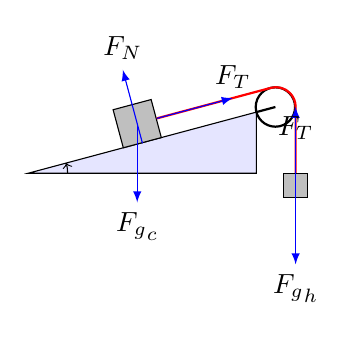
\begin{tikzpicture}[force/.style={>=latex,draw=blue,fill=blue},plane/.style={draw=black,fill=blue!10},string/.style={draw=red, thick},pulley/.style={thick},M/.style={rectangle,draw,fill=lightgray,minimum size=0.5cm,thin},m/.style={rectangle,draw=black,fill=lightgray,minimum size=0.3cm,thin},]
        \draw[plane] (0,-1) coordinate (base)
        -- coordinate[pos=0.5] (mid) ++(15:3) coordinate (top)
        |- (base) -- cycle;
        \path (mid) node[M,rotate=15,yshift=0.25cm] (M) {};
        \draw[pulley] (top) -- ++(15:0.25) circle (0.25cm)
        ++ (90-15:0.5) coordinate (pulley);
        \draw[string] (M.east) -- ++(15:1.5cm) arc (90+15:0:0.25)
        -- ++(0,-1) node[m] (m) {};

        \draw [force,->] (M.center) -- ++(0,-1) node[below] {${F_g}_c$};
        \begin{scope}[rotate=15]
            \draw [force,->] (M.south) -- ++(0,{cos(15)}) node[above] {$F_N$};
            \draw [force,->] (M.east) -- ++(1,0) node[above] {$F_T$};
        \end{scope}

        \draw [force,->] (m.center) -- ++(0,-1) node[below] {${F_g}_h$};
        \draw [force,->] (m.center) -- ++(0,1) node[below] {$F_T$};

        \draw[->] (base)++(0.5cm,0) arc (0:15:0.5cm);
    \end{tikzpicture}
\end{center}
\section{Derivations}
Starting with:
\[\Delta x = v_0t + \frac{1}{2}at^2\]
Since $\Delta x$ is $d$ and $v_0$ is 0, this can be simplified to:
\[d = \frac{1}{2}at^2\]
Solving for $a$, we obtain:
\[a = \frac{2d}{t^2}\]
\subsection{Uphill}
Replacing $F_{net} = ma$ with $F_{net}$ and $a$, we obtain:
\[m_hg - m_cg\sin(\theta) = (m_h + m_c)\frac{2d}{t^2}\]
Solving for $m_h$, we obtain:
\[m_h = \frac{m_cg\sin(\theta) + \frac{2m_cd}{t^2}}{g - \frac{2d}{t^2}}\]
\subsection{Downhill}
Replacing $F_{net} = ma$ with $F_{net}$ and $a$, we obtain:
\[m_cg\sin(\theta) - m_hg = (m_h + m_c)\frac{2d}{t^2}\]
Solving for $m_h$, we obtain:
\[m_h = \frac{m_cg\sin(\theta) - \frac{2m_cd}{t^2}}{g + \frac{2d}{t^2}}\]
\section{Data}
Trial 1 was the uphill trial, and Trial 2 was the downhill trial.
\begin{center}
    \pgfplotstabletypeset[col sep=comma, precision=2, every head row/.style={
                before row={
                        \toprule
                    },
                after row={
                        \bottomrule
                    },
            },
        every last row/.style={
                after row=\bottomrule
            }]{Lab 2.2.csv}
\end{center}
\end{document}